\documentclass[10pt,twocolumn,letterpaper]{article}

\usepackage{iccv}
\usepackage{times}
\usepackage{epsfig}
\usepackage{graphicx}
\usepackage{amsmath}
\usepackage{amssymb}

% Include other packages here, before hyperref.

% If you comment hyperref and then uncomment it, you should delete
% egpaper.aux before re-running latex.  (Or just hit 'q' on the first latex
% run, let it finish, and you should be clear).
\usepackage[breaklinks=true,bookmarks=false]{hyperref}

\iccvfinalcopy % *** Uncomment this line for the final submission

\def\iccvPaperID{****} % *** Enter the ICCV Paper ID here
\def\httilde{\mbox{\tt\raisebox{-.5ex}{\symbol{126}}}}

% Pages are numbered in submission mode, and unnumbered in camera-ready
%\ificcvfinal\pagestyle{empty}\fi
\setcounter{page}{4321}
\begin{document}

%%%%%%%%% TITLE
\title{Handwritten Digits Classification by Support Vector Machine}

\author{Huihuang Zheng\\
UTEID: hz4674\\
{\tt\small huihuang@utexas.edu}
% For a paper whose authors are all at the same institution,
% omit the following lines up until the closing ``}''.
% Additional authors and addresses can be added with ``\and'',
% just like the second author.
% To save space, use either the email address or home page, not both
%\and
%Second Author\\
%Institution2\\
%First line of institution2 address\\
%{\tt\small secondauthor@i2.org}
}

\maketitle
%\thispagestyle{empty}


%%%%%%%%% ABSTRACT
\begin{abstract}
  Support Vector Machine (SVM) \cite{cortes1995support} is a powerful technic in machine learning. In this work, we explore what factors can influence the accuracy of SVM in handwritten digit classification accuracy. We found that Principal Component Analysis (PCA) \cite{jolliffe2002principal}, applying image features (e.g. Histogram of Histograms of Oriented Gradients, HOG \cite{dalal2005histograms}), increasing the number of Eigenvectors, and increasing size of training data can significantly improve the accuracy. We also find training images used for PCA doesn't effect the SVM accuracy much. Finally, we found SVM kernel types can effect the SVM accuracy and number of images need to be used for training.
\end{abstract}

\section{Implementation}
\subsection{Pre-required Software and Tools}
In this work, we used Matlab. Our SVM tool is from LIBSVM \cite{CC01a} and we used library VLFeat \cite{vedaldi08vlfeat} for computing image feature Histograms of Oriented Gradients (HOG) \cite{dalal2005histograms}. LIBSVM has executable files and we attached them in \textbf{./src} so you don't need to install them. But you need to have Matlab in your computer and install VLFeat to your Matlab.

\subsection{Implementation Details}
\subsubsection{Pre-computing Image Features}
see \textbf{./src/precomputeImageFeatures.m}. Pre-compute image features and store them into file will make experiments faster because you don't need to re-compute image features every time you run an experiment. This function just calls interface of VLFeat \cite{vedaldi08vlfeat}.


\subsubsection{Baseline Experiments}
see \textbf{./src/baselineExperiment.m}. We use SVM on raw image data, without PCA, linear kernel: u'*v to run experiment as baseline. The function changes the sizes used for training SVM and call LIBSVM interface: libsvmtrain, libsvmpredict to train SVM and get accuracy.
\subsubsection{SVM Experiments interface}
see \textbf{./src/svmExperiment.m}. The function firstly converts the image into features (by loading pre-computed features or compute now, in this work, we computed feature of HOG \cite{dalal2005histograms} using cell size 4), then pick exact number of images as SVM training set. In the SVM data, the function pick specific number of images as PCA training set. The pick method is change first $n$ images. Then, it's PCA step. We call the code in homework1 to get eigenvectors and mean of PCA training data. Next, we project training and testing data to eigenvectors space ( subtract mean from training and testing data and then multiply the eigenvectors). After we have done PCA, we convert training data into LIBSVM input format and rescale training and testing data to range $[0, 1]$. Finally, we call LIBSVM interface: libsvmtrain, libsvmpredict to train and get accuracy and write results to output file.

\subsubsection{Main Function}
see \textbf{./src/main/m}. The function specified the path for data files, the different parameters we used for experiments and run the \textbf{baselineExperiment.m} and \textbf{svmExperiment.m} with different parameters.

\subsection{Run my code}
see \textbf{./readme.txt} for running instructions. Note that it takes a few minutes to train and test by SVM. Running all experiments in \textbf{./src/main/m} costs about 1.5 hour. (not including pre-computing of features). Pre-computing features take about 3 hours. I attached pre-computing features in uploaded code so you don't need to run pre-computing feature step.

\section{Experiment}
To see how different parameters influence accuracy of SVM classification, we fixed some parameters and changed some parameters.

\subsection{How do PCA and Image Features and Training Size of SVM influence the SVM accuracy?}
Our experiment result is presented in the following table. The Img Feature can be hog (HOG \cite{dalal2005histograms}) or raw (raw image). The experiment uses linear kernel of SVM ($x' * y$), 600 images to train PCA and use 50 eigenvectors. Table \ref{t1} and Figure \ref{f1} show impact of PCA and HOG features. We could see that without PCA and HOG feature, we simple apply SVM in the images just got 9.74\% accuracy. Even random guess can get 10\% accuracy, so SVM without PCA cannot be applied to images. Then, by comparing PCA + Raw and PCA + HOG, we could find the HOG feature improve a lot of SVM accuracy. Since PCA and HOG can help a lot, all my following experiments will use PCA + HOG.
\begin{table}

    \begin{tabular}{|c|c|c|c|}
      \hline
      Using PCA & Img Feature & Train Size & Accuracy \\
      \hline
      no & raw & 1000 & 0.0974 \\
      no & raw & 10000 & 0.0974 \\
      no & raw & 60000 & 0.0974 \\
      \hline
      yes & raw & 1000 & 0.8587 \\
      yes & raw & 10000 & 0.9082 \\
      yes & raw & 60000 & 0.9244 \\
      \hline
      yes & hog & 1000 & 0.9474 \\
      yea & hog & 10000 & 0.9737 \\
      yes & hog & 60000 & 0.9796 \\
      \hline
    \end{tabular}
    \caption{Impact of PCA and HOG feature}
    \label{t1}
\end{table}


\begin{figure}
  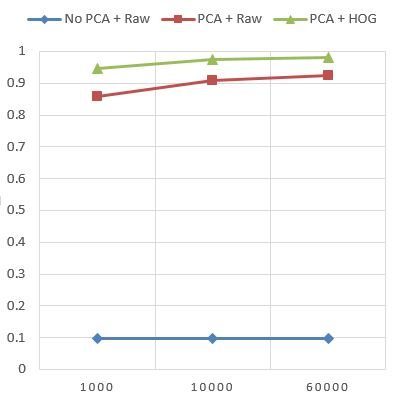
\includegraphics[width=0.95\linewidth]{f1.JPG}
  \caption{Impact of PCA and HOG feature}
  \label{f1}
\end{figure}

\subsection{How does training size of PCA influence the SVM accuracy?}
In this experiment, we use PCA + HOG, 60000 images to train SVM with linear kernel ($x' * y$), different numbers of images to train PCA and using first 50 eigenvectors. The result is presented in Table \ref{t2}. From the result, we could see that with increasing sizes of PCA training, the accuracy of SVM can increase or decrease. So once you train PCA enough, you don't need a lot of images to run PCA because increasing number of training doesn't always have positive effect.

\begin{table}

    \begin{center}
    \begin{tabular}{|c|c|}
      \hline
      PCA Training Size & Accuracy \\
      \hline
        250	& 0.9815 \\
        300	& 0.9786 \\
        350	& 0.9781 \\
        400	& 0.9725 \\
        450	& 0.9775 \\
        500	& 0.977 \\
        550	& 0.9823 \\
        600	& 0.9796 \\
      \hline
    \end{tabular}
    \end{center}
    \caption{Impact of PCA training size}
    \label{t2}
\end{table}

\subsection{How does number of eigenvectors influence the SVM accuracy?}
In this experiment, we use PCA + HOG, 60000 images to train SVM with linear kernel ($x' * y$), 600 images to train PCA but use different number of eigenvectors. We increased number of eigenvectors we used from 10 to 80 with increment of 10. We could see using more eigenvectors in PCA can increase the SVM accuracy.

\begin{table}
    \begin{center}
    \begin{tabular}{|c|c|}
      \hline
      Number of Eigenvectors & Accuracy \\
      \hline
        10 & 0.9241\\
        20 & 0.9666\\
        30 & 0.9769\\
        40 & 0.978 \\
        50 & 0.9796\\
        60 & 0.9822\\
        70 & 0.982 \\
        80 & 0.9841\\
      \hline
    \end{tabular}
    \end{center}
    \caption{Impact of number of eigenvectors}
    \label{t3}
\end{table}

\begin{figure}
  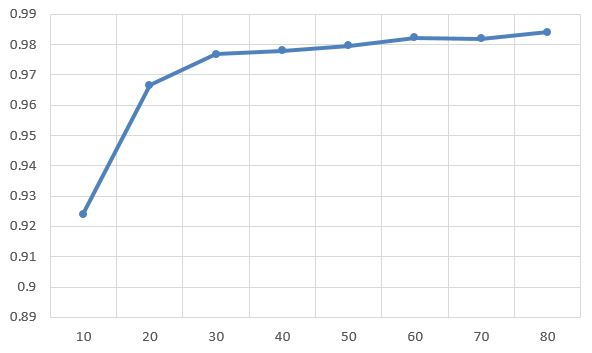
\includegraphics[width=0.95\linewidth]{f2.JPG}
  \caption{Impact of number of eigenvectors}
  \label{f2}
\end{figure}

\subsection{Different Kernels}
In this experiment, we compare four types of kernels. 1, linear: $x' * y$. 2, polynomial: $ ( x' * y ) ^ 3 $. 3, radial basis: $\exp(-\gamma * |x-y| ^2)$. 4, sigmoid: $\tanh(\gamma * x' * y)$. In radial basis and sigmoid kernels $\gamma = 1/number\_of\_features$. The result was presented in Table \ref{t4} and Figure \ref{f3}. Although when we use all 60000 training images, those kernels can all achieve accuracy between 96\% and 98\%, the polynomial and sigmoid kernels can not got high accuracy when we only use 1000 training data. So you need more data to let polynomial and sigmoid kernels get high accuracy. So we can see different kind of kernels not only influence accuracy but also how many data you need to train the SVM. 

 
\begin{table}
    \begin{center}
    \begin{tabular}{|c|c|c|}
      \hline
      Kernel & SVM Train Size & Accuracy \\
      \hline
      linear & 1000 & 0.9474 \\
      linear & 10000 & 0.9737 \\
      linear & 60000 & 0.9796 \\
      \hline
      polynomial & 1000 & 0.1028 \\
      polynomial & 10000 & 0.8965 \\
      polynomial & 60000 & 0.9642\\
      \hline
      radial & 1000 & 0.9105 \\
      radial & 10000 & 0.9654 \\
      radial & 60000 & 0.9755 \\
      \hline
      sigmoid & 1000 & 0.4359 \\
      sigmoid & 10000 & 0.9611 \\
      sigmoid & 60000 & 0.9729 \\
      \hline
    \end{tabular}
    \end{center}
    
    \caption{Impact of Different Kernels}
    \label{t4}
\end{table}

\begin{figure}
  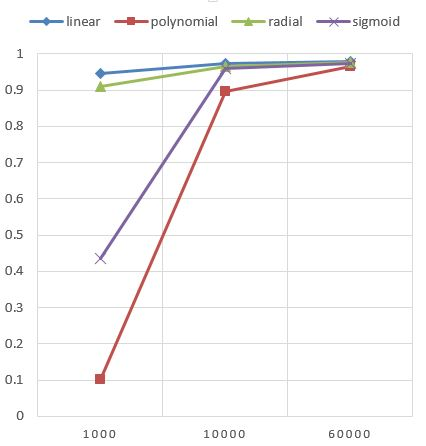
\includegraphics[width=0.95\linewidth]{f3.JPG}
  \caption{Impact of Different Kernels}
  \label{f3}
\end{figure}

\section{Conclusion}
In this work, we explore what factors can influence the accuracy of SVM in handwritten digit classification accuracy. We found that Principal Component Analysis (PCA) \cite{jolliffe2002principal}, applying image features (e.g. Histogram of Histograms of Oriented Gradients, HOG \cite{dalal2005histograms}), increasing the number of Eigenvectors, and increasing size of training data can significantly improve the accuracy. We also find training images used for PCA doesn't effect the SVM accuracy much. Finally, we found SVM kernel types can effect the SVM accuracy and number of images need to be used for training.
%%%%%%%%% BODY TEXT


{\small
\bibliographystyle{ieee}
\bibliography{egbib}
}

\end{document}
